\chapter[Conclusion]{Conclusion}
\label{Chap:Conclusion}


\section{Limitations and improvements}

\begin{itemize}
    \item Bidirectional filtering - currently only doing incomming filtering
    \item Support IPv6
    \item Redesign of the transmit logic to consume less resources while not losing on speed/performance - can reduce number of buffers. 
    \item Add a second interface - would need a new pcb and would need onboard switch if webserver was also wanted.
    \item Utilise the DDR2 RAM onboard the Nexys a7 board for RAM to free up BRAM. 
    \item Use another FPGA board with only the essential peripherals (eg dont need USB, Audio, temperature sensor etc on Nexys board)
    \item Support certificates for HTTPS. 
    \item Support faster media interfaces, eg RGMII for 1Gbit/s or XGMII for 10Gbit/s as an example
    \item Make efficiency considerations in the ethernet hardware and RISC-V core. 
\end{itemize}


If a second interface was added, you'd have to design a seperate board as the Nexys A7 board only has one ethernet PHY and the additional PMOD ports are not suitable for ethernet. This is because the PMOD ports are only rated for a 25Mhz bandwidth, while the RMII signals are 50Mhz. As such, signal integrity issues arose (see figure \ref{fig:eye_diagram}) and restricted the use to just one interface - the onboard PHY. A new development board with two PHYs would be needed.

\begin{figure}[h]
    \centering
    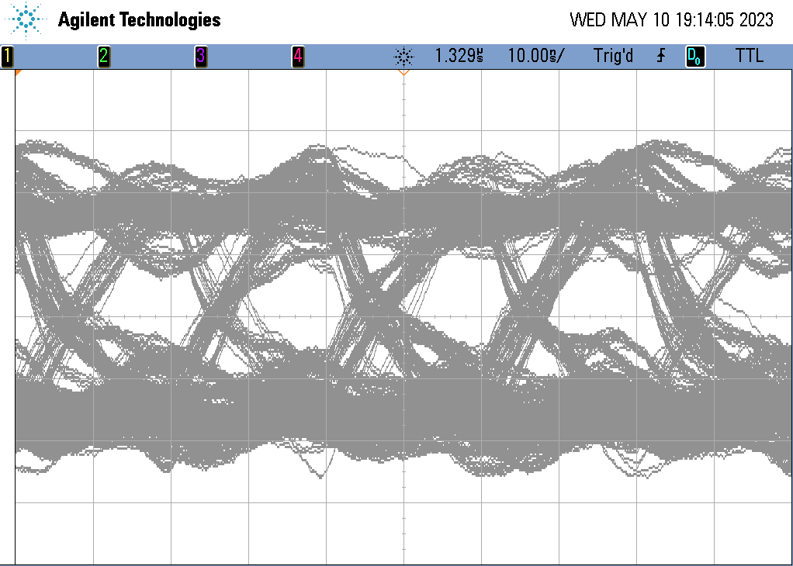
\includegraphics[width=0.65\textwidth]{Images/EyeDiagramTX.png}
    \caption[Eye diagram of TXD through PMOD interface]{Eye diagram of TXD through PMOD interface.}
    \label{fig:eye_diagram}
\end{figure}




\section{Recommendations}

Add dedicated hardware packet filtering to SoC based computers - safer - faster, efficient and lightweight

Reduce number of transmit buffers needed - consolidate them.

Use an FPGA with more BRAM as this would help with filter sizes, buffers and also ram needed for the RTOS and webservers.

Consider Hybrid SoC FPGA such as the Xilinx Zynq lineup.

Hardware ethernet and packet filter reduces latency, but is bottlenecked by CPU.

Use a different bus which the processor can handle - wishbone is overkill ~2.5Gbit for 100Mbit connection.

If power efficiency is desired, consider something like the MilkV duo. 128mA at 94mbit/s

The NeoRV32 is a solid softcore processor, but it's size grows exponentially when you use the wishbone interface. It's feature set is growing and while good, is not a great idea in production devices. 


While Freertos plus TCP provides a good library, it's documentation and community support is lackluster in comparison to LwIP. But is relatively easy to use. 
 
Using Vue.js to write the website in is a good idea as it reduces the network traffic between the device as routing is handled on the client side. So for lightweight applications, it is ideal. No need to have a special webserver for it as the site is static. However a separate API is needed, but easy to implement. 


Configure the DHCP server so that it statically assigns the IP address to the firewall for easy configuration. 


\section{Sustainability}

Ethernet standards have been in place since xxxx and the IP, TCP, UDP and other layer 4 protocols have been in service for decades and have not changed. Typically if new features do need to be added in these areas, they are added ontop of and not modify the packet structure itself. Such event was in 1998 with the introduction of IPv6 \cite{rfc2460}.

While malicious bad actors come up with new and innovative ways to breach a system, the core of this packet filter is solid and fundamentally should not need to change in future. Instead other additions to the architecture of a system should be added to better protect a host. 

Using the neorv32 while is feature-rich, as it's in its developement process and new features are continually getting added and existing features moved around, it doesn't make for the best choice for ease of updating, but it does get regularly updated so if there was a security vulnerability, odds are that it will get patched.

Perhaps a larger issue with sustainability is the lifecyle of a Vue.js webapp. When updates are needed, potentially new versions of the toolchain may be needed thus contributing to longer development times. 

Choice of riscv makes this project easy to commercialise since there is no licences needed for the risc-v cores are royalty free and the specific variant, neorv32 is open sourced under the BSD-3-Clause license. \footnote[1]{See: https://github.com/stnolting/neorv32/blob/main/LICENSE}

This design was deployed on a Xilinx Artix 7 FPGA board with the LAN8720A PHY. As the LAN8720A chip uses the standardised RMII interface, there should be no issues porting the project to another FPGA or FPGA board so long as there is sufficient LUTs and BRAM available on the FPGA and uses an RMII phy. The hardware could be updated to RGMII or XGMII without too many issues with the main difference being in the input and output FIFO being able to support the different clock rates and bit widths.  


\section{Future work}

